% Created by tikzDevice version 0.10.1 on 2016-11-22 07:08:32
% !TEX encoding = UTF-8 Unicode
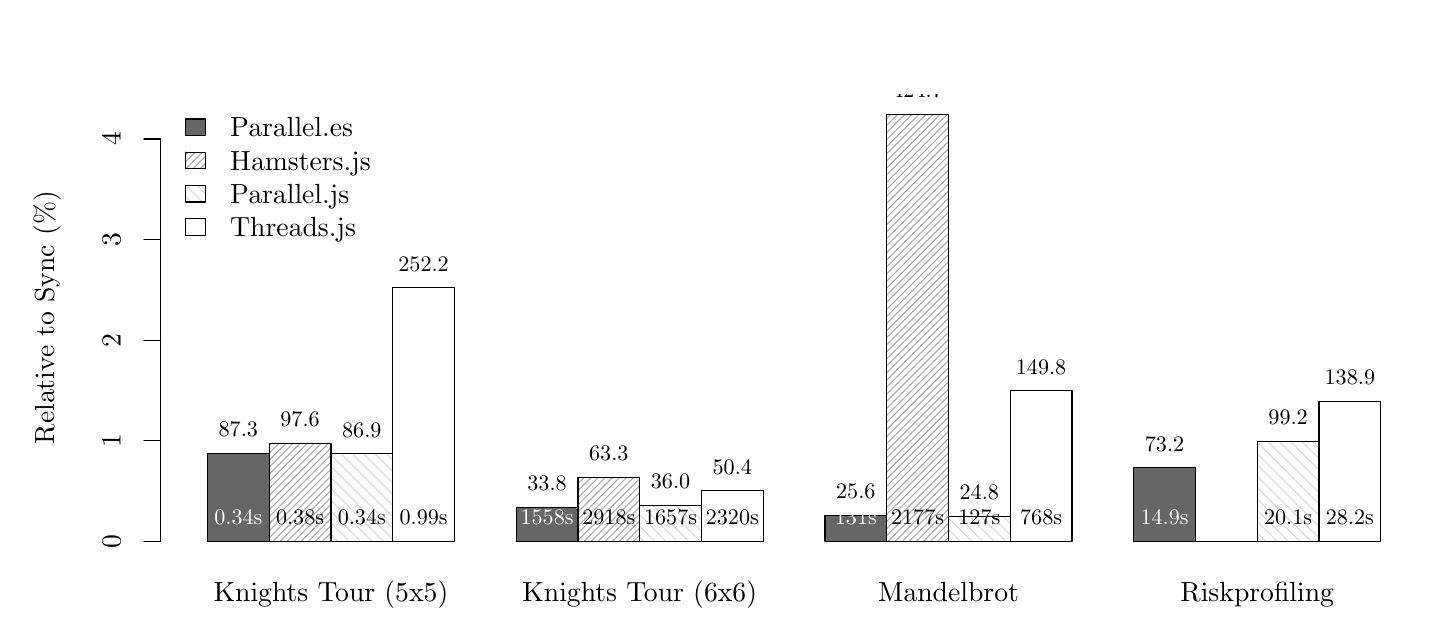
\begin{tikzpicture}[x=1pt,y=1pt]
\definecolor{fillColor}{RGB}{255,255,255}
\path[use as bounding box,fill=fillColor,fill opacity=0.00] (0,0) rectangle (505.89,209.58);
\begin{scope}
\path[clip] (  0.00,  0.00) rectangle (505.89,209.58);
\definecolor{fillColor}{gray}{0.40}

\path[fill=fillColor] ( 64.96, 24.00) --
	( 87.27, 24.00) --
	( 87.27, 55.72) --
	( 64.96, 55.72) --
	cycle;
\definecolor{drawColor}{RGB}{172,172,172}

\path[draw=drawColor,line width= 0.4pt,line join=round,line cap=round] ( 87.27, 58.41) -- ( 88.33, 59.47);

\path[draw=drawColor,line width= 0.4pt,line join=round,line cap=round] ( 87.27, 55.85) -- ( 90.89, 59.47);

\path[draw=drawColor,line width= 0.4pt,line join=round,line cap=round] ( 87.27, 53.30) -- ( 93.44, 59.47);

\path[draw=drawColor,line width= 0.4pt,line join=round,line cap=round] ( 87.27, 50.74) -- ( 96.00, 59.47);

\path[draw=drawColor,line width= 0.4pt,line join=round,line cap=round] ( 87.27, 48.19) -- ( 98.55, 59.47);

\path[draw=drawColor,line width= 0.4pt,line join=round,line cap=round] ( 87.27, 45.63) -- (101.11, 59.47);

\path[draw=drawColor,line width= 0.4pt,line join=round,line cap=round] ( 87.27, 43.08) -- (103.66, 59.47);

\path[draw=drawColor,line width= 0.4pt,line join=round,line cap=round] ( 87.27, 40.52) -- (106.22, 59.47);

\path[draw=drawColor,line width= 0.4pt,line join=round,line cap=round] ( 87.27, 37.97) -- (108.77, 59.47);

\path[draw=drawColor,line width= 0.4pt,line join=round,line cap=round] ( 87.27, 35.41) -- (109.59, 57.73);

\path[draw=drawColor,line width= 0.4pt,line join=round,line cap=round] ( 87.27, 32.86) -- (109.59, 55.17);

\path[draw=drawColor,line width= 0.4pt,line join=round,line cap=round] ( 87.27, 30.30) -- (109.59, 52.62);

\path[draw=drawColor,line width= 0.4pt,line join=round,line cap=round] ( 87.27, 27.75) -- (109.59, 50.06);

\path[draw=drawColor,line width= 0.4pt,line join=round,line cap=round] ( 87.27, 25.19) -- (109.59, 47.51);

\path[draw=drawColor,line width= 0.4pt,line join=round,line cap=round] ( 88.64, 24.00) -- (109.59, 44.95);

\path[draw=drawColor,line width= 0.4pt,line join=round,line cap=round] ( 91.19, 24.00) -- (109.59, 42.40);

\path[draw=drawColor,line width= 0.4pt,line join=round,line cap=round] ( 93.75, 24.00) -- (109.59, 39.84);

\path[draw=drawColor,line width= 0.4pt,line join=round,line cap=round] ( 96.30, 24.00) -- (109.59, 37.29);

\path[draw=drawColor,line width= 0.4pt,line join=round,line cap=round] ( 98.86, 24.00) -- (109.59, 34.73);

\path[draw=drawColor,line width= 0.4pt,line join=round,line cap=round] (101.41, 24.00) -- (109.59, 32.17);

\path[draw=drawColor,line width= 0.4pt,line join=round,line cap=round] (103.97, 24.00) -- (109.59, 29.62);

\path[draw=drawColor,line width= 0.4pt,line join=round,line cap=round] (106.52, 24.00) -- (109.59, 27.06);

\path[draw=drawColor,line width= 0.4pt,line join=round,line cap=round] (109.08, 24.00) -- (109.59, 24.51);
\definecolor{drawColor}{RGB}{218,218,218}

\path[draw=drawColor,line width= 0.4pt,line join=round,line cap=round] (112.14, 24.00) -- (109.59, 26.56);

\path[draw=drawColor,line width= 0.4pt,line join=round,line cap=round] (116.23, 24.00) -- (109.59, 30.64);

\path[draw=drawColor,line width= 0.4pt,line join=round,line cap=round] (120.32, 24.00) -- (109.59, 34.73);

\path[draw=drawColor,line width= 0.4pt,line join=round,line cap=round] (124.41, 24.00) -- (109.59, 38.82);

\path[draw=drawColor,line width= 0.4pt,line join=round,line cap=round] (128.50, 24.00) -- (109.59, 42.91);

\path[draw=drawColor,line width= 0.4pt,line join=round,line cap=round] (131.90, 24.68) -- (109.59, 47.00);

\path[draw=drawColor,line width= 0.4pt,line join=round,line cap=round] (131.90, 28.77) -- (109.59, 51.09);

\path[draw=drawColor,line width= 0.4pt,line join=round,line cap=round] (131.90, 32.86) -- (109.59, 55.17);

\path[draw=drawColor,line width= 0.4pt,line join=round,line cap=round] (131.90, 36.95) -- (113.27, 55.58);

\path[draw=drawColor,line width= 0.4pt,line join=round,line cap=round] (131.90, 41.04) -- (117.36, 55.58);

\path[draw=drawColor,line width= 0.4pt,line join=round,line cap=round] (131.90, 45.12) -- (121.45, 55.58);

\path[draw=drawColor,line width= 0.4pt,line join=round,line cap=round] (131.90, 49.21) -- (125.54, 55.58);

\path[draw=drawColor,line width= 0.4pt,line join=round,line cap=round] (131.90, 53.30) -- (129.62, 55.58);

\path[fill=fillColor] (176.53, 24.00) --
	(198.84, 24.00) --
	(198.84, 36.29) --
	(176.53, 36.29) --
	cycle;
\definecolor{drawColor}{RGB}{172,172,172}

\path[draw=drawColor,line width= 0.4pt,line join=round,line cap=round] (198.84, 44.78) -- (201.08, 47.02);

\path[draw=drawColor,line width= 0.4pt,line join=round,line cap=round] (198.84, 42.22) -- (203.64, 47.02);

\path[draw=drawColor,line width= 0.4pt,line join=round,line cap=round] (198.84, 39.67) -- (206.19, 47.02);

\path[draw=drawColor,line width= 0.4pt,line join=round,line cap=round] (198.84, 37.11) -- (208.75, 47.02);

\path[draw=drawColor,line width= 0.4pt,line join=round,line cap=round] (198.84, 34.56) -- (211.30, 47.02);

\path[draw=drawColor,line width= 0.4pt,line join=round,line cap=round] (198.84, 32.00) -- (213.86, 47.02);

\path[draw=drawColor,line width= 0.4pt,line join=round,line cap=round] (198.84, 29.45) -- (216.41, 47.02);

\path[draw=drawColor,line width= 0.4pt,line join=round,line cap=round] (198.84, 26.89) -- (218.97, 47.02);

\path[draw=drawColor,line width= 0.4pt,line join=round,line cap=round] (198.84, 24.34) -- (221.16, 46.65);

\path[draw=drawColor,line width= 0.4pt,line join=round,line cap=round] (201.06, 24.00) -- (221.16, 44.10);

\path[draw=drawColor,line width= 0.4pt,line join=round,line cap=round] (203.62, 24.00) -- (221.16, 41.54);

\path[draw=drawColor,line width= 0.4pt,line join=round,line cap=round] (206.17, 24.00) -- (221.16, 38.99);

\path[draw=drawColor,line width= 0.4pt,line join=round,line cap=round] (208.73, 24.00) -- (221.16, 36.43);

\path[draw=drawColor,line width= 0.4pt,line join=round,line cap=round] (211.28, 24.00) -- (221.16, 33.88);

\path[draw=drawColor,line width= 0.4pt,line join=round,line cap=round] (213.84, 24.00) -- (221.16, 31.32);

\path[draw=drawColor,line width= 0.4pt,line join=round,line cap=round] (216.39, 24.00) -- (221.16, 28.77);

\path[draw=drawColor,line width= 0.4pt,line join=round,line cap=round] (218.95, 24.00) -- (221.16, 26.21);
\definecolor{drawColor}{RGB}{218,218,218}

\path[draw=drawColor,line width= 0.4pt,line join=round,line cap=round] (222.53, 24.00) -- (221.16, 25.37);

\path[draw=drawColor,line width= 0.4pt,line join=round,line cap=round] (226.61, 24.00) -- (221.16, 29.45);

\path[draw=drawColor,line width= 0.4pt,line join=round,line cap=round] (230.70, 24.00) -- (221.16, 33.54);

\path[draw=drawColor,line width= 0.4pt,line join=round,line cap=round] (234.79, 24.00) -- (221.72, 37.07);

\path[draw=drawColor,line width= 0.4pt,line join=round,line cap=round] (238.88, 24.00) -- (225.81, 37.07);

\path[draw=drawColor,line width= 0.4pt,line join=round,line cap=round] (242.97, 24.00) -- (229.90, 37.07);

\path[draw=drawColor,line width= 0.4pt,line join=round,line cap=round] (243.47, 27.58) -- (233.99, 37.07);

\path[draw=drawColor,line width= 0.4pt,line join=round,line cap=round] (243.47, 31.67) -- (238.07, 37.07);

\path[draw=drawColor,line width= 0.4pt,line join=round,line cap=round] (243.47, 35.76) -- (242.16, 37.07);

\path[fill=fillColor] (288.10, 24.00) --
	(310.42, 24.00) --
	(310.42, 33.30) --
	(288.10, 33.30) --
	cycle;
\definecolor{drawColor}{RGB}{172,172,172}

\path[draw=drawColor,line width= 0.4pt,line join=round,line cap=round] (310.42,176.79) -- (311.94,178.32);

\path[draw=drawColor,line width= 0.4pt,line join=round,line cap=round] (310.42,174.24) -- (314.50,178.32);

\path[draw=drawColor,line width= 0.4pt,line join=round,line cap=round] (310.42,171.68) -- (317.05,178.32);

\path[draw=drawColor,line width= 0.4pt,line join=round,line cap=round] (310.42,169.13) -- (319.61,178.32);

\path[draw=drawColor,line width= 0.4pt,line join=round,line cap=round] (310.42,166.57) -- (322.16,178.32);

\path[draw=drawColor,line width= 0.4pt,line join=round,line cap=round] (310.42,164.02) -- (324.72,178.32);

\path[draw=drawColor,line width= 0.4pt,line join=round,line cap=round] (310.42,161.46) -- (327.27,178.32);

\path[draw=drawColor,line width= 0.4pt,line join=round,line cap=round] (310.42,158.91) -- (329.83,178.32);

\path[draw=drawColor,line width= 0.4pt,line join=round,line cap=round] (310.42,156.35) -- (332.38,178.32);

\path[draw=drawColor,line width= 0.4pt,line join=round,line cap=round] (310.42,153.79) -- (332.73,176.11);

\path[draw=drawColor,line width= 0.4pt,line join=round,line cap=round] (310.42,151.24) -- (332.73,173.55);

\path[draw=drawColor,line width= 0.4pt,line join=round,line cap=round] (310.42,148.68) -- (332.73,171.00);

\path[draw=drawColor,line width= 0.4pt,line join=round,line cap=round] (310.42,146.13) -- (332.73,168.44);

\path[draw=drawColor,line width= 0.4pt,line join=round,line cap=round] (310.42,143.57) -- (332.73,165.89);

\path[draw=drawColor,line width= 0.4pt,line join=round,line cap=round] (310.42,141.02) -- (332.73,163.33);

\path[draw=drawColor,line width= 0.4pt,line join=round,line cap=round] (310.42,138.46) -- (332.73,160.78);

\path[draw=drawColor,line width= 0.4pt,line join=round,line cap=round] (310.42,135.91) -- (332.73,158.22);

\path[draw=drawColor,line width= 0.4pt,line join=round,line cap=round] (310.42,133.35) -- (332.73,155.67);

\path[draw=drawColor,line width= 0.4pt,line join=round,line cap=round] (310.42,130.80) -- (332.73,153.11);

\path[draw=drawColor,line width= 0.4pt,line join=round,line cap=round] (310.42,128.24) -- (332.73,150.56);

\path[draw=drawColor,line width= 0.4pt,line join=round,line cap=round] (310.42,125.69) -- (332.73,148.00);

\path[draw=drawColor,line width= 0.4pt,line join=round,line cap=round] (310.42,123.13) -- (332.73,145.45);

\path[draw=drawColor,line width= 0.4pt,line join=round,line cap=round] (310.42,120.58) -- (332.73,142.89);

\path[draw=drawColor,line width= 0.4pt,line join=round,line cap=round] (310.42,118.02) -- (332.73,140.34);

\path[draw=drawColor,line width= 0.4pt,line join=round,line cap=round] (310.42,115.47) -- (332.73,137.78);

\path[draw=drawColor,line width= 0.4pt,line join=round,line cap=round] (310.42,112.91) -- (332.73,135.23);

\path[draw=drawColor,line width= 0.4pt,line join=round,line cap=round] (310.42,110.36) -- (332.73,132.67);

\path[draw=drawColor,line width= 0.4pt,line join=round,line cap=round] (310.42,107.80) -- (332.73,130.12);

\path[draw=drawColor,line width= 0.4pt,line join=round,line cap=round] (310.42,105.25) -- (332.73,127.56);

\path[draw=drawColor,line width= 0.4pt,line join=round,line cap=round] (310.42,102.69) -- (332.73,125.01);

\path[draw=drawColor,line width= 0.4pt,line join=round,line cap=round] (310.42,100.14) -- (332.73,122.45);

\path[draw=drawColor,line width= 0.4pt,line join=round,line cap=round] (310.42, 97.58) -- (332.73,119.90);

\path[draw=drawColor,line width= 0.4pt,line join=round,line cap=round] (310.42, 95.03) -- (332.73,117.34);

\path[draw=drawColor,line width= 0.4pt,line join=round,line cap=round] (310.42, 92.47) -- (332.73,114.79);

\path[draw=drawColor,line width= 0.4pt,line join=round,line cap=round] (310.42, 89.92) -- (332.73,112.23);

\path[draw=drawColor,line width= 0.4pt,line join=round,line cap=round] (310.42, 87.36) -- (332.73,109.68);

\path[draw=drawColor,line width= 0.4pt,line join=round,line cap=round] (310.42, 84.81) -- (332.73,107.12);

\path[draw=drawColor,line width= 0.4pt,line join=round,line cap=round] (310.42, 82.25) -- (332.73,104.57);

\path[draw=drawColor,line width= 0.4pt,line join=round,line cap=round] (310.42, 79.70) -- (332.73,102.01);

\path[draw=drawColor,line width= 0.4pt,line join=round,line cap=round] (310.42, 77.14) -- (332.73, 99.46);

\path[draw=drawColor,line width= 0.4pt,line join=round,line cap=round] (310.42, 74.59) -- (332.73, 96.90);

\path[draw=drawColor,line width= 0.4pt,line join=round,line cap=round] (310.42, 72.03) -- (332.73, 94.35);

\path[draw=drawColor,line width= 0.4pt,line join=round,line cap=round] (310.42, 69.48) -- (332.73, 91.79);

\path[draw=drawColor,line width= 0.4pt,line join=round,line cap=round] (310.42, 66.92) -- (332.73, 89.23);

\path[draw=drawColor,line width= 0.4pt,line join=round,line cap=round] (310.42, 64.37) -- (332.73, 86.68);

\path[draw=drawColor,line width= 0.4pt,line join=round,line cap=round] (310.42, 61.81) -- (332.73, 84.12);

\path[draw=drawColor,line width= 0.4pt,line join=round,line cap=round] (310.42, 59.26) -- (332.73, 81.57);

\path[draw=drawColor,line width= 0.4pt,line join=round,line cap=round] (310.42, 56.70) -- (332.73, 79.01);

\path[draw=drawColor,line width= 0.4pt,line join=round,line cap=round] (310.42, 54.14) -- (332.73, 76.46);

\path[draw=drawColor,line width= 0.4pt,line join=round,line cap=round] (310.42, 51.59) -- (332.73, 73.90);

\path[draw=drawColor,line width= 0.4pt,line join=round,line cap=round] (310.42, 49.03) -- (332.73, 71.35);

\path[draw=drawColor,line width= 0.4pt,line join=round,line cap=round] (310.42, 46.48) -- (332.73, 68.79);

\path[draw=drawColor,line width= 0.4pt,line join=round,line cap=round] (310.42, 43.92) -- (332.73, 66.24);

\path[draw=drawColor,line width= 0.4pt,line join=round,line cap=round] (310.42, 41.37) -- (332.73, 63.68);

\path[draw=drawColor,line width= 0.4pt,line join=round,line cap=round] (310.42, 38.81) -- (332.73, 61.13);

\path[draw=drawColor,line width= 0.4pt,line join=round,line cap=round] (310.42, 36.26) -- (332.73, 58.57);

\path[draw=drawColor,line width= 0.4pt,line join=round,line cap=round] (310.42, 33.70) -- (332.73, 56.02);

\path[draw=drawColor,line width= 0.4pt,line join=round,line cap=round] (310.42, 31.15) -- (332.73, 53.46);

\path[draw=drawColor,line width= 0.4pt,line join=round,line cap=round] (310.42, 28.59) -- (332.73, 50.91);

\path[draw=drawColor,line width= 0.4pt,line join=round,line cap=round] (310.42, 26.04) -- (332.73, 48.35);

\path[draw=drawColor,line width= 0.4pt,line join=round,line cap=round] (310.93, 24.00) -- (332.73, 45.80);

\path[draw=drawColor,line width= 0.4pt,line join=round,line cap=round] (313.49, 24.00) -- (332.73, 43.24);

\path[draw=drawColor,line width= 0.4pt,line join=round,line cap=round] (316.04, 24.00) -- (332.73, 40.69);

\path[draw=drawColor,line width= 0.4pt,line join=round,line cap=round] (318.60, 24.00) -- (332.73, 38.13);

\path[draw=drawColor,line width= 0.4pt,line join=round,line cap=round] (321.15, 24.00) -- (332.73, 35.58);

\path[draw=drawColor,line width= 0.4pt,line join=round,line cap=round] (323.71, 24.00) -- (332.73, 33.02);

\path[draw=drawColor,line width= 0.4pt,line join=round,line cap=round] (326.26, 24.00) -- (332.73, 30.47);

\path[draw=drawColor,line width= 0.4pt,line join=round,line cap=round] (328.82, 24.00) -- (332.73, 27.91);

\path[draw=drawColor,line width= 0.4pt,line join=round,line cap=round] (331.37, 24.00) -- (332.73, 25.36);
\definecolor{drawColor}{RGB}{218,218,218}

\path[draw=drawColor,line width= 0.4pt,line join=round,line cap=round] (332.91, 24.00) -- (332.73, 24.18);

\path[draw=drawColor,line width= 0.4pt,line join=round,line cap=round] (337.00, 24.00) -- (332.73, 28.26);

\path[draw=drawColor,line width= 0.4pt,line join=round,line cap=round] (341.08, 24.00) -- (332.73, 32.35);

\path[draw=drawColor,line width= 0.4pt,line join=round,line cap=round] (345.17, 24.00) -- (336.17, 33.00);

\path[draw=drawColor,line width= 0.4pt,line join=round,line cap=round] (349.26, 24.00) -- (340.26, 33.00);

\path[draw=drawColor,line width= 0.4pt,line join=round,line cap=round] (353.35, 24.00) -- (344.35, 33.00);

\path[draw=drawColor,line width= 0.4pt,line join=round,line cap=round] (355.05, 26.39) -- (348.44, 33.00);

\path[draw=drawColor,line width= 0.4pt,line join=round,line cap=round] (355.05, 30.48) -- (352.52, 33.00);

\path[fill=fillColor] (399.67, 24.00) --
	(421.99, 24.00) --
	(421.99, 50.60) --
	(399.67, 50.60) --
	cycle;
\definecolor{drawColor}{RGB}{172,172,172}

\path[draw=drawColor,line width= 0.4pt,line join=round,line cap=round] (423.36, 24.00) -- (423.36, 24.00);

\path[draw=drawColor,line width= 0.4pt,line join=round,line cap=round] (425.91, 24.00) -- (425.91, 24.00);

\path[draw=drawColor,line width= 0.4pt,line join=round,line cap=round] (428.47, 24.00) -- (428.47, 24.00);

\path[draw=drawColor,line width= 0.4pt,line join=round,line cap=round] (431.02, 24.00) -- (431.02, 24.00);

\path[draw=drawColor,line width= 0.4pt,line join=round,line cap=round] (433.58, 24.00) -- (433.58, 24.00);

\path[draw=drawColor,line width= 0.4pt,line join=round,line cap=round] (436.13, 24.00) -- (436.13, 24.00);

\path[draw=drawColor,line width= 0.4pt,line join=round,line cap=round] (438.69, 24.00) -- (438.69, 24.00);

\path[draw=drawColor,line width= 0.4pt,line join=round,line cap=round] (441.24, 24.00) -- (441.24, 24.00);

\path[draw=drawColor,line width= 0.4pt,line join=round,line cap=round] (443.80, 24.00) -- (443.80, 24.00);
\definecolor{drawColor}{RGB}{218,218,218}

\path[draw=drawColor,line width= 0.4pt,line join=round,line cap=round] (447.38, 24.00) -- (444.30, 27.07);

\path[draw=drawColor,line width= 0.4pt,line join=round,line cap=round] (451.47, 24.00) -- (444.30, 31.16);

\path[draw=drawColor,line width= 0.4pt,line join=round,line cap=round] (455.55, 24.00) -- (444.30, 35.25);

\path[draw=drawColor,line width= 0.4pt,line join=round,line cap=round] (459.64, 24.00) -- (444.30, 39.34);

\path[draw=drawColor,line width= 0.4pt,line join=round,line cap=round] (463.73, 24.00) -- (444.30, 43.43);

\path[draw=drawColor,line width= 0.4pt,line join=round,line cap=round] (466.62, 25.20) -- (444.30, 47.52);

\path[draw=drawColor,line width= 0.4pt,line join=round,line cap=round] (466.62, 29.29) -- (444.30, 51.60);

\path[draw=drawColor,line width= 0.4pt,line join=round,line cap=round] (466.62, 33.38) -- (444.30, 55.69);

\path[draw=drawColor,line width= 0.4pt,line join=round,line cap=round] (466.62, 37.47) -- (444.30, 59.78);

\path[draw=drawColor,line width= 0.4pt,line join=round,line cap=round] (466.62, 41.55) -- (448.14, 60.03);

\path[draw=drawColor,line width= 0.4pt,line join=round,line cap=round] (466.62, 45.64) -- (452.23, 60.03);

\path[draw=drawColor,line width= 0.4pt,line join=round,line cap=round] (466.62, 49.73) -- (456.32, 60.03);

\path[draw=drawColor,line width= 0.4pt,line join=round,line cap=round] (466.62, 53.82) -- (460.41, 60.03);

\path[draw=drawColor,line width= 0.4pt,line join=round,line cap=round] (466.62, 57.91) -- (464.49, 60.03);
\definecolor{drawColor}{RGB}{0,0,0}

\path[draw=drawColor,line width= 0.4pt,line join=round,line cap=round] ( 64.96, 24.00) --
	( 87.27, 24.00) --
	( 87.27, 55.72) --
	( 64.96, 55.72) --
	( 64.96, 24.00);

\path[draw=drawColor,line width= 0.4pt,line join=round,line cap=round] ( 87.27, 24.00) --
	(109.59, 24.00) --
	(109.59, 59.47) --
	( 87.27, 59.47) --
	( 87.27, 24.00);

\path[draw=drawColor,line width= 0.4pt,line join=round,line cap=round] (109.59, 24.00) --
	(131.90, 24.00) --
	(131.90, 55.58) --
	(109.59, 55.58) --
	(109.59, 24.00);

\path[draw=drawColor,line width= 0.4pt,line join=round,line cap=round] (131.90, 24.00) --
	(154.22, 24.00) --
	(154.22,115.63) --
	(131.90,115.63) --
	(131.90, 24.00);

\path[draw=drawColor,line width= 0.4pt,line join=round,line cap=round] (176.53, 24.00) --
	(198.84, 24.00) --
	(198.84, 36.29) --
	(176.53, 36.29) --
	(176.53, 24.00);

\path[draw=drawColor,line width= 0.4pt,line join=round,line cap=round] (198.84, 24.00) --
	(221.16, 24.00) --
	(221.16, 47.02) --
	(198.84, 47.02) --
	(198.84, 24.00);

\path[draw=drawColor,line width= 0.4pt,line join=round,line cap=round] (221.16, 24.00) --
	(243.47, 24.00) --
	(243.47, 37.07) --
	(221.16, 37.07) --
	(221.16, 24.00);

\path[draw=drawColor,line width= 0.4pt,line join=round,line cap=round] (243.47, 24.00) --
	(265.79, 24.00) --
	(265.79, 42.30) --
	(243.47, 42.30) --
	(243.47, 24.00);

\path[draw=drawColor,line width= 0.4pt,line join=round,line cap=round] (288.10, 24.00) --
	(310.42, 24.00) --
	(310.42, 33.30) --
	(288.10, 33.30) --
	(288.10, 24.00);

\path[draw=drawColor,line width= 0.4pt,line join=round,line cap=round] (310.42, 24.00) --
	(332.73, 24.00) --
	(332.73,178.32) --
	(310.42,178.32) --
	(310.42, 24.00);

\path[draw=drawColor,line width= 0.4pt,line join=round,line cap=round] (332.73, 24.00) --
	(355.05, 24.00) --
	(355.05, 33.00) --
	(332.73, 33.00) --
	(332.73, 24.00);

\path[draw=drawColor,line width= 0.4pt,line join=round,line cap=round] (355.05, 24.00) --
	(377.36, 24.00) --
	(377.36, 78.43) --
	(355.05, 78.43) --
	(355.05, 24.00);

\path[draw=drawColor,line width= 0.4pt,line join=round,line cap=round] (399.67, 24.00) --
	(421.99, 24.00) --
	(421.99, 50.60) --
	(399.67, 50.60) --
	(399.67, 24.00);

\path[draw=drawColor,line width= 0.4pt,line join=round,line cap=round] (421.99, 24.00) --
	(444.30, 24.00) --
	(421.99, 24.00);

\path[draw=drawColor,line width= 0.4pt,line join=round,line cap=round] (444.30, 24.00) --
	(466.62, 24.00) --
	(466.62, 60.03) --
	(444.30, 60.03) --
	(444.30, 24.00);

\path[draw=drawColor,line width= 0.4pt,line join=round,line cap=round] (466.62, 24.00) --
	(488.93, 24.00) --
	(488.93, 74.49) --
	(466.62, 74.49) --
	(466.62, 24.00);
\end{scope}
\begin{scope}
\path[clip] (  0.00,  0.00) rectangle (505.89,209.58);
\definecolor{drawColor}{RGB}{0,0,0}

\node[text=drawColor,anchor=base,inner sep=0pt, outer sep=0pt, scale=  1.00] at (109.59,  2.40) {Knights Tour (5x5)};

\node[text=drawColor,anchor=base,inner sep=0pt, outer sep=0pt, scale=  1.00] at (221.16,  2.40) {Knights Tour (6x6)};

\node[text=drawColor,anchor=base,inner sep=0pt, outer sep=0pt, scale=  1.00] at (332.73,  2.40) {Mandelbrot};

\node[text=drawColor,anchor=base,inner sep=0pt, outer sep=0pt, scale=  1.00] at (444.30,  2.40) {Riskprofiling};
\end{scope}
\begin{scope}
\path[clip] (  0.00,  0.00) rectangle (505.89,209.58);
\definecolor{drawColor}{RGB}{0,0,0}

\node[text=drawColor,rotate= 90.00,anchor=base,inner sep=0pt, outer sep=0pt, scale=  1.00] at (  9.60,104.79) {Relative to Sync ({\%})};
\end{scope}
\begin{scope}
\path[clip] (  0.00,  0.00) rectangle (505.89,209.58);
\definecolor{drawColor}{RGB}{0,0,0}

\path[draw=drawColor,line width= 0.4pt,line join=round,line cap=round] ( 48.00, 24.00) -- ( 48.00,169.34);

\path[draw=drawColor,line width= 0.4pt,line join=round,line cap=round] ( 48.00, 24.00) -- ( 42.00, 24.00);

\path[draw=drawColor,line width= 0.4pt,line join=round,line cap=round] ( 48.00, 60.33) -- ( 42.00, 60.33);

\path[draw=drawColor,line width= 0.4pt,line join=round,line cap=round] ( 48.00, 96.67) -- ( 42.00, 96.67);

\path[draw=drawColor,line width= 0.4pt,line join=round,line cap=round] ( 48.00,133.00) -- ( 42.00,133.00);

\path[draw=drawColor,line width= 0.4pt,line join=round,line cap=round] ( 48.00,169.34) -- ( 42.00,169.34);

\node[text=drawColor,rotate= 90.00,anchor=base,inner sep=0pt, outer sep=0pt, scale=  1.00] at ( 33.60, 24.00) {0};

\node[text=drawColor,rotate= 90.00,anchor=base,inner sep=0pt, outer sep=0pt, scale=  1.00] at ( 33.60, 60.33) {1};

\node[text=drawColor,rotate= 90.00,anchor=base,inner sep=0pt, outer sep=0pt, scale=  1.00] at ( 33.60, 96.67) {2};

\node[text=drawColor,rotate= 90.00,anchor=base,inner sep=0pt, outer sep=0pt, scale=  1.00] at ( 33.60,133.00) {3};

\node[text=drawColor,rotate= 90.00,anchor=base,inner sep=0pt, outer sep=0pt, scale=  1.00] at ( 33.60,169.34) {4};
\end{scope}
\begin{scope}
\path[clip] ( 48.00, 24.00) rectangle (505.89,185.58);
\definecolor{fillColor}{gray}{0.40}

\path[fill=fillColor] ( 57.00,176.58) --
	( 64.20,176.58) --
	( 64.20,170.58) --
	( 57.00,170.58) --
	cycle;
\definecolor{drawColor}{RGB}{172,172,172}

\path[draw=drawColor,line width= 0.4pt,line join=round,line cap=round] ( 57.00,163.56) -- ( 58.03,164.58);

\path[draw=drawColor,line width= 0.4pt,line join=round,line cap=round] ( 57.00,161.00) -- ( 60.58,164.58);

\path[draw=drawColor,line width= 0.4pt,line join=round,line cap=round] ( 57.14,158.58) -- ( 63.14,164.58);

\path[draw=drawColor,line width= 0.4pt,line join=round,line cap=round] ( 59.69,158.58) -- ( 64.20,163.09);

\path[draw=drawColor,line width= 0.4pt,line join=round,line cap=round] ( 62.25,158.58) -- ( 64.20,160.54);
\definecolor{drawColor}{RGB}{218,218,218}

\path[draw=drawColor,line width= 0.4pt,line join=round,line cap=round] ( 59.06,146.58) -- ( 57.00,148.64);

\path[draw=drawColor,line width= 0.4pt,line join=round,line cap=round] ( 63.15,146.58) -- ( 57.15,152.58);

\path[draw=drawColor,line width= 0.4pt,line join=round,line cap=round] ( 64.20,149.62) -- ( 61.24,152.58);
\definecolor{drawColor}{RGB}{0,0,0}

\path[draw=drawColor,line width= 0.4pt,line join=round,line cap=round] ( 57.00,176.58) --
	( 64.20,176.58) --
	( 64.20,170.58) --
	( 57.00,170.58) --
	( 57.00,176.58);

\path[draw=drawColor,line width= 0.4pt,line join=round,line cap=round] ( 57.00,164.58) --
	( 64.20,164.58) --
	( 64.20,158.58) --
	( 57.00,158.58) --
	( 57.00,164.58);

\path[draw=drawColor,line width= 0.4pt,line join=round,line cap=round] ( 57.00,152.58) --
	( 64.20,152.58) --
	( 64.20,146.58) --
	( 57.00,146.58) --
	( 57.00,152.58);

\path[draw=drawColor,line width= 0.4pt,line join=round,line cap=round] ( 57.00,140.58) --
	( 64.20,140.58) --
	( 64.20,134.58) --
	( 57.00,134.58) --
	( 57.00,140.58);

\node[text=drawColor,anchor=base west,inner sep=0pt, outer sep=0pt, scale=  1.00] at ( 73.20,170.14) {Parallel.es};

\node[text=drawColor,anchor=base west,inner sep=0pt, outer sep=0pt, scale=  1.00] at ( 73.20,158.14) {Hamsters.js};

\node[text=drawColor,anchor=base west,inner sep=0pt, outer sep=0pt, scale=  1.00] at ( 73.20,146.14) {Parallel.js};

\node[text=drawColor,anchor=base west,inner sep=0pt, outer sep=0pt, scale=  1.00] at ( 73.20,134.14) {Threads.js};

\node[text=drawColor,anchor=base,inner sep=0pt, outer sep=0pt, scale=  0.80] at ( 76.12, 61.72) {87.3};

\node[text=drawColor,anchor=base,inner sep=0pt, outer sep=0pt, scale=  0.80] at ( 98.43, 65.47) {97.6};

\node[text=drawColor,anchor=base,inner sep=0pt, outer sep=0pt, scale=  0.80] at (120.74, 61.58) {86.9};

\node[text=drawColor,anchor=base,inner sep=0pt, outer sep=0pt, scale=  0.80] at (143.06,121.63) {252.2};

\node[text=drawColor,anchor=base,inner sep=0pt, outer sep=0pt, scale=  0.80] at (187.69, 42.29) {33.8};

\node[text=drawColor,anchor=base,inner sep=0pt, outer sep=0pt, scale=  0.80] at (210.00, 53.02) {63.3};

\node[text=drawColor,anchor=base,inner sep=0pt, outer sep=0pt, scale=  0.80] at (232.32, 43.07) {36.0};

\node[text=drawColor,anchor=base,inner sep=0pt, outer sep=0pt, scale=  0.80] at (254.63, 48.30) {50.4};

\node[text=drawColor,anchor=base,inner sep=0pt, outer sep=0pt, scale=  0.80] at (299.26, 39.30) {25.6};

\node[text=drawColor,anchor=base,inner sep=0pt, outer sep=0pt, scale=  0.80] at (321.57,184.32) {424.7};

\node[text=drawColor,anchor=base,inner sep=0pt, outer sep=0pt, scale=  0.80] at (343.89, 39.00) {24.8};

\node[text=drawColor,anchor=base,inner sep=0pt, outer sep=0pt, scale=  0.80] at (366.20, 84.43) {149.8};

\node[text=drawColor,anchor=base,inner sep=0pt, outer sep=0pt, scale=  0.80] at (410.83, 56.60) {73.2};

\node[text=drawColor,anchor=base,inner sep=0pt, outer sep=0pt, scale=  0.80] at (455.46, 66.03) {99.2};

\node[text=drawColor,anchor=base,inner sep=0pt, outer sep=0pt, scale=  0.80] at (477.77, 80.49) {138.9};
\definecolor{drawColor}{RGB}{255,255,255}

\node[text=drawColor,anchor=base,inner sep=0pt, outer sep=0pt, scale=  0.80] at ( 76.12, 30.00) {0.34s};
\definecolor{drawColor}{RGB}{0,0,0}

\node[text=drawColor,anchor=base,inner sep=0pt, outer sep=0pt, scale=  0.80] at ( 98.43, 30.00) {0.38s};

\node[text=drawColor,anchor=base,inner sep=0pt, outer sep=0pt, scale=  0.80] at (120.74, 30.00) {0.34s};

\node[text=drawColor,anchor=base,inner sep=0pt, outer sep=0pt, scale=  0.80] at (143.06, 30.00) {0.99s};
\definecolor{drawColor}{RGB}{255,255,255}

\node[text=drawColor,anchor=base,inner sep=0pt, outer sep=0pt, scale=  0.80] at (187.69, 30.00) {1558s};
\definecolor{drawColor}{RGB}{0,0,0}

\node[text=drawColor,anchor=base,inner sep=0pt, outer sep=0pt, scale=  0.80] at (210.00, 30.00) {2918s};

\node[text=drawColor,anchor=base,inner sep=0pt, outer sep=0pt, scale=  0.80] at (232.32, 30.00) {1657s};

\node[text=drawColor,anchor=base,inner sep=0pt, outer sep=0pt, scale=  0.80] at (254.63, 30.00) {2320s};
\definecolor{drawColor}{RGB}{255,255,255}

\node[text=drawColor,anchor=base,inner sep=0pt, outer sep=0pt, scale=  0.80] at (299.26, 30.00) {131s};
\definecolor{drawColor}{RGB}{0,0,0}

\node[text=drawColor,anchor=base,inner sep=0pt, outer sep=0pt, scale=  0.80] at (321.57, 30.00) {2177s};

\node[text=drawColor,anchor=base,inner sep=0pt, outer sep=0pt, scale=  0.80] at (343.89, 30.00) {127s};

\node[text=drawColor,anchor=base,inner sep=0pt, outer sep=0pt, scale=  0.80] at (366.20, 30.00) {768s};
\definecolor{drawColor}{RGB}{255,255,255}

\node[text=drawColor,anchor=base,inner sep=0pt, outer sep=0pt, scale=  0.80] at (410.83, 30.00) {14.9s};
\definecolor{drawColor}{RGB}{0,0,0}

\node[text=drawColor,anchor=base,inner sep=0pt, outer sep=0pt, scale=  0.80] at (455.46, 30.00) {20.1s};

\node[text=drawColor,anchor=base,inner sep=0pt, outer sep=0pt, scale=  0.80] at (477.77, 30.00) {28.2s};
\end{scope}
\end{tikzpicture}
